\chapter{Supporting Information: Effect of Quantum Delocalization on Temperature 
Dependent Double Proton Transfer in Molecular Crystals of Terephthalic Acid} \label{appendix4}

\section{0K structure of the three forms of Terephthalic Acid}
\label{form-si}

As mentioned in Chapter-3, Terephthalic acid exists in three polymorphs, namely, form I, II and 
III. While the lowest energy one, i.e., form I has been described in Chapter-3, here we discuss
the results of form II and III. Figure~\ref{fig:cip1} and \ref{fig:cip2} show the structure of form II
and III respectively. The main difference between form I and the other forms is the stacking of the
two layers. While in form II, the -COOH groups of two molecules in a chain that are involved in 
H-bonding, are stacked above the benzene ring of TPA in the layer below it, in form I and III, the
molecules are perfectly stacked on top of each other. Additionally, in form I and II there are
improper weak interchain H-bonds. Compared to form I, in form III, two neighbouring chains are shifted
with respect to one another thereby disrupting the interchain C-H$\cdots$O H-bonds. This also results in doubling of the cell size in form III. Table~\ref{tab:0K_str} compares our computed values of lattice
parameters with the experimental results. We found that they are in reasonably good agreement.
Further, from the computation of the cohesive energy, we find that while they are similar in form I
and II, the TPA molecules are weakly bound in form III.  

\begin{table}
    \centering
    \begin{tabular}{|*{9}{c|}}
     \hline
     Form & a& b & c& $\alpha$ & $\beta$ & $\gamma$ & Vol.&$\Delta E^{coh}$\\ 
           & (\AA)& (\AA) & (\AA)& ($^{\circ}$) & ($^{\circ}$) & ($^{\circ}$) & (\AA$^3$) &(eV/mol.)\\ \hline
        I & 9.625 & 7.606 & 3.623 & 73.80 & 105.07 & 139.44 & 165.13&1.811 \\
        I-exp\cite{bailey1967crystal}& 9.54 & 7.73 & 3.75 & 70.85 & 107.36 & 137.78 & 174.76& \\ \hline
               
        II & 9.623 & 5.247 &  4.945 & 85.76 & 136.10 & 104.36 & 165.17&1.809 \\
        II-exp\cite{bailey1967crystal}& 9.54 & 5.34 & 5.02 & 86.95 & 134.65 & 104.90 & 172.77& \\ \hline

        III &  8.899 & 10.449 & 3.612 & 86.30 & 89.36 & 91.06& 335.12&1.748 \\ 
        III-exp\cite{sledz2001new}& 8.940& 10.442 & 3.79 & 90.0 & 91.21 & 90.0 & 353.72& \\ \hline

    \end{tabular}
    \caption{Comparison of the lattice parameters and cohesive energies ($\Delta E^{coh}$) of the three polymorphs of TPA.}
    \label{tab:0K_str}
\end{table}

\begin{figure}
    \centering
    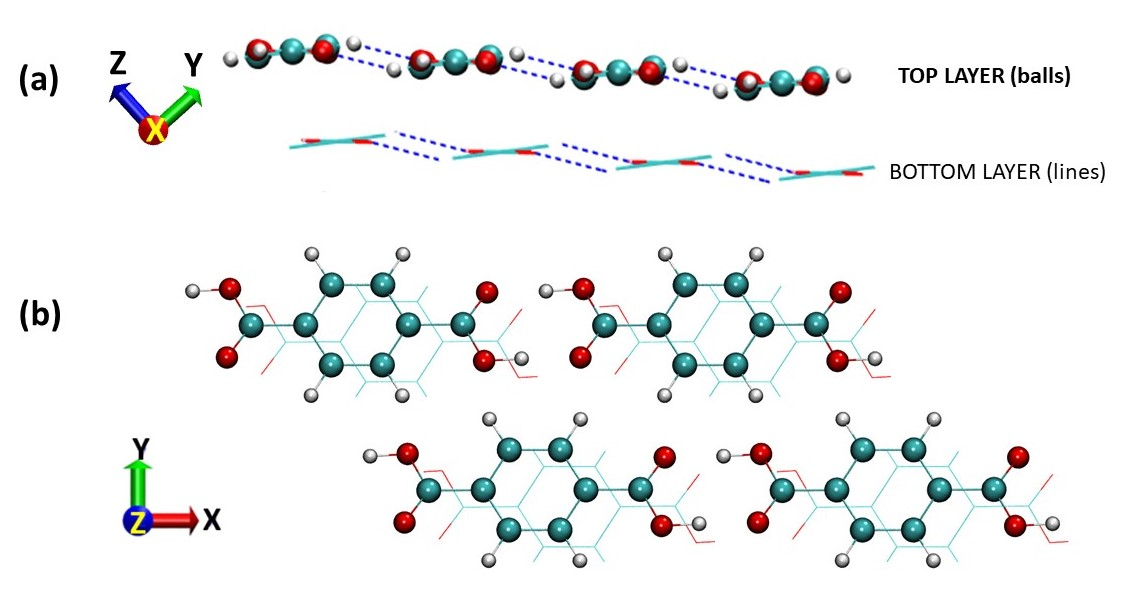
\includegraphics[width=15cm ]{./Appendix4/new_figures_si/figure0.jpg}
    \caption{Crystal structure representation of TPA (form I) using ball and stick representation. (a) Side view (along the chain axis) represents the stacking of molecular chains (b) Top view (along z axis) shows layer-layer overlap. Top layer atoms in solid balls and bottom layer atoms as points. Green, red and white balls represent carbon, oxygen and hydrogen respectively}
    \label{fig:cip0}
\end{figure}

\begin{figure}
    \centering
    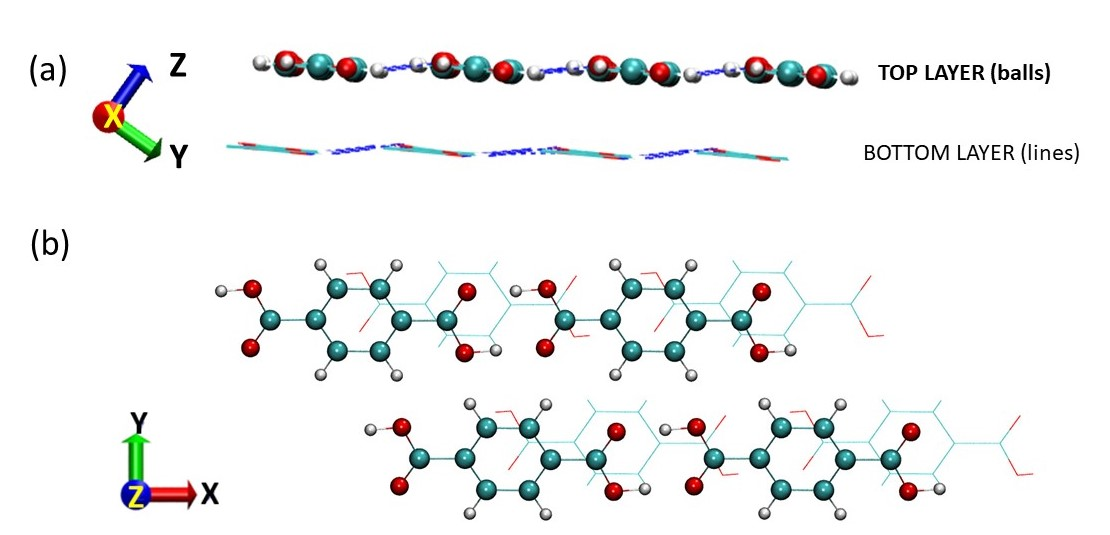
\includegraphics[width=15cm ]{./Appendix4/new_figures_si/figure1.jpg}
    \caption{Crystal structure representation of TPA (form II) using ball and stick representation. (a) Side view (along the chain axis) represents the stacking of molecular chains (b) Top view (along z axis) shows layer-layer overlap. Top layer atoms in solid balls and bottom layer atoms as points. Green, red and white balls represent carbon, oxygen and hydrogen respectively.}
    \label{fig:cip1}
\end{figure}

\begin{figure}
    \centering
    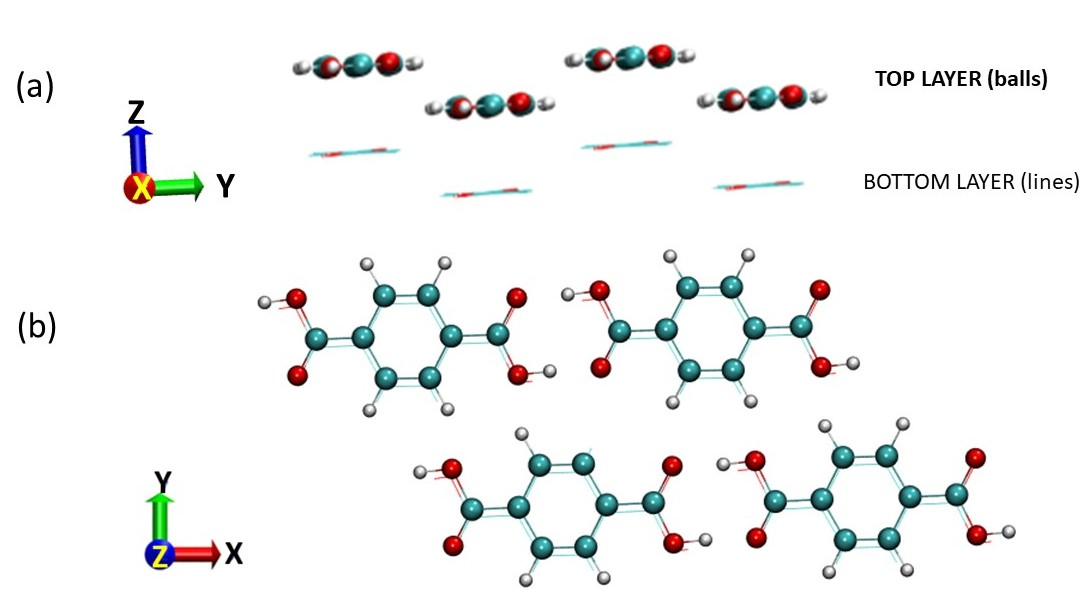
\includegraphics[width=15cm ]{./Appendix4/new_figures_si/figure2.jpg}
    \caption{Crystal structure representation of TPA (form III) using ball and stick representation. (a) Side view (along the chain axis) represents the stacking of two molecular chains (b) Top view (along z axis) shows layer-layer overlap. Top layer atoms in solid balls and bottom layer atoms as points. Green, red and white balls represent carbon, oxygen and hydrogen respectively.}
    \label{fig:cip2}
\end{figure}

\section{Convergence of PIGLET simulation w.r.t the number of beads}
\label{convergence_si}
PIGLET simulations use path integral formulation of statistical mechanics to incorporate NQE. In this approach, the quantum nucleus is transformed into a classical ring polymer of ``$P$" beads/imaginary time slices where each bead is connected to (two) neighbouring beads through harmonic potential. In the limit $P \rightarrow  \infty$,  the transformation is exact and gives accurate quantum statistics of the nuclear system. However, in reality only a finite number of beads are used. Hence, it is
necessary to perform convergence tests of the relevant properties with respect to the number of beads.
Since the number of beads is inversely proportional to the temperature, convergence tests 
need to be performed at the lowest simulation temperature. In our study 70 K is the lowest temperature. Therefore, we have performed convergence test of the following thermodynamic quantities with respect to the number of beads at 70 K:
(i) potential energy (Figure \ref{fig:cip7}(a)) and (ii) quantum kinetic Energy (Figure 
\ref{fig:cip7}(b)). The convergence tests were conducted on 4, 12, 16, 24, 32 and 64 beads where 4 and
12 beads were sampled for 5 ps and the others for 10 ps. The potential and quantum kinetic energy 
(per atom) converged at 16 beads. 

\begin{figure}
    \centering
    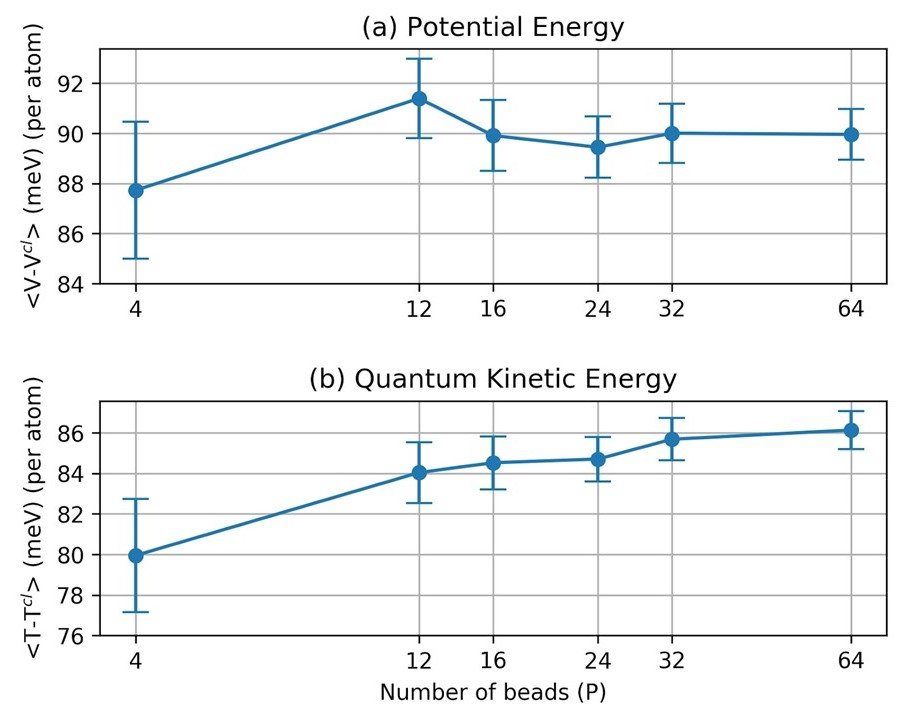
\includegraphics[width=15cm ]{./Appendix4/new_figures_si/figure7.jpg}
    \caption{ Potential energy (top panel) and quantum kinetic energy (bottom panel) as a function of the number of beads.}
    \label{fig:cip7}
\end{figure}

The convergence obtained for the thermodynamic quantities does not guarantee the accurate description 
of system properties. Hence, additional convergence tests were undertaken for quantities related to 
the investigation of proton transfers along the hydrogen bond. These are (i) the 
heavy atom distance ($d_{O-O}$, Figure \ref{fig:cip8}(a)), (ii) the hydrogen bond angle 
($\angle$O-H-O, Figure \ref{fig:cip8}(b)), (iii) the radius of gyration of the proton ($r_G$, Figure 
\ref{fig:cip8}(c)) and (iv) the the effective free energy as a function of proton transfer coordinates
($\delta_1$ and $\delta_2$, Figure \ref{fig:cip9}). 

The converged number of beads for $d_{O-O}$ and  $\angle$O-H-O is at 12 whereas the $r_G$ needs 16 
beads to achieve convergence. The effective free energy as a function of the proton transfer 
coordinates needs a higher value of 64 beads. The reason for the distribution to not converge has to 
do with the fact that the proportion of the transferring hydrogen atom decreases as the number of 
beads increases. This is observed because $P$ is directly proportional to the force constant of the 
inter bead harmonic potential. Consequently, an increase in the number of beads slows the sampling of 
the potential energy landscape and would require longer simulation time. Therefore, an overall 
comparison for all the beads would not be completely relevant to check the convergence as we focus 
mainly on the nature of the proton transfer.  In order to compare the nature of a specific proton 
transfer, i.e., whether the proton hops or tunnels, the radius of gyration as a function of sampling time is compared with the time evolution of
the centroid proton transfer coordinate. The graphs at the two values of ``$P$" (16 and 64) are shown 
in Figure \ref{fig:cip10}. It is observed that the nature of transfer does not change when the number of 
beads is increased from 16 to 64. Hence, 16 beads were used for the PIGLET simulations at all 
temperatures.  

\begin{figure}
    \centering
    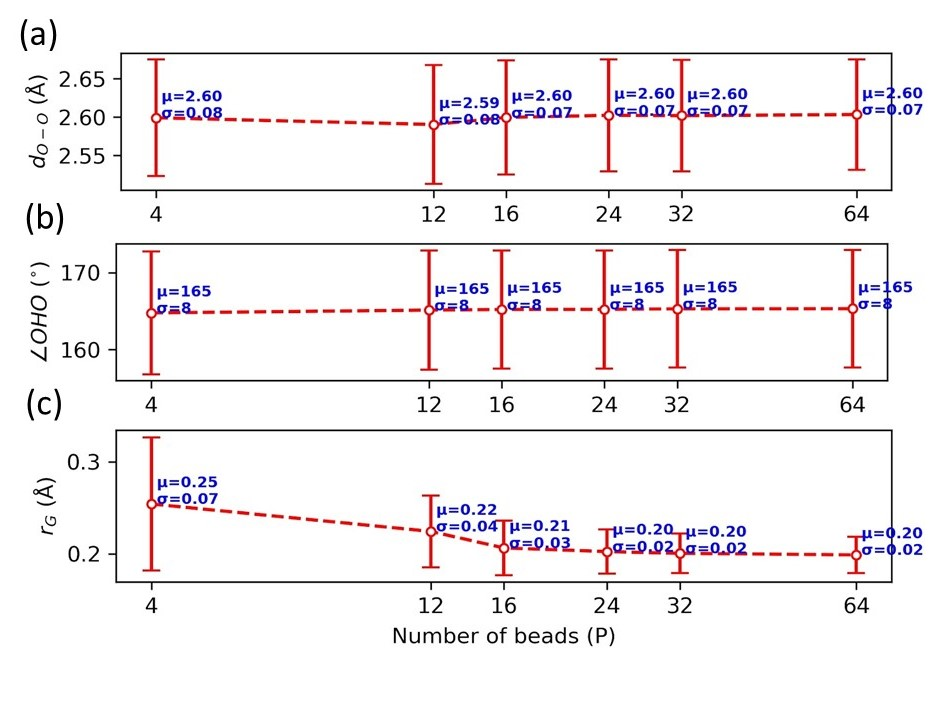
\includegraphics[width=15cm ]{./Appendix4/new_figures_si/figure8.jpg}
    \caption{Convergence with respect to the number of beads for (a) the heavy atom separation ($d_{O-O}$), (b) the hydrogen bond angle,($\angle$O-H-O) and (c) the radius of gyration of the O-H hydrogen ($r_G$).}
    \label{fig:cip8}
\end{figure}

\begin{figure}
    \centering
    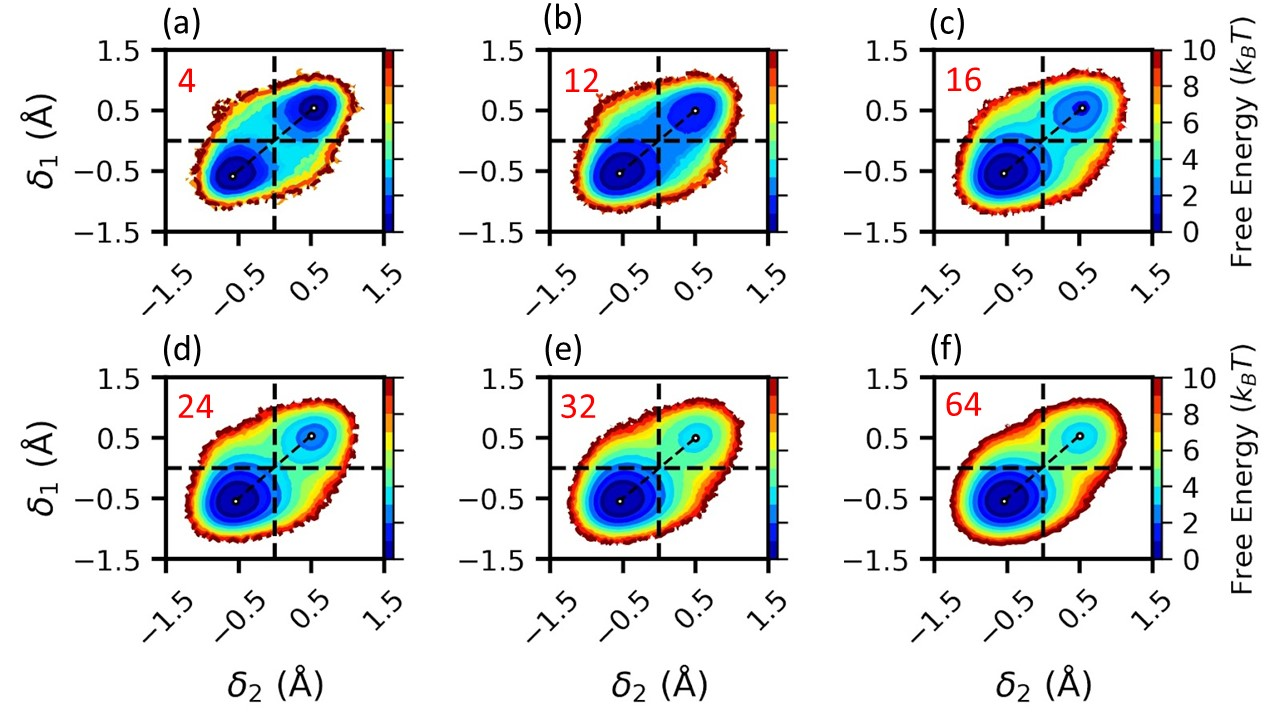
\includegraphics[width=15cm ]{./Appendix4/new_figures_si/figure9.jpg}
    \caption{The effective free energy as a function of the proton transfer
coordinates $\delta_1$ and $\delta_2$ for (a-f) 4, 12, 16, 24, 32 and 64 beads.}
    \label{fig:cip9}
\end{figure}

\begin{figure}
    \centering
    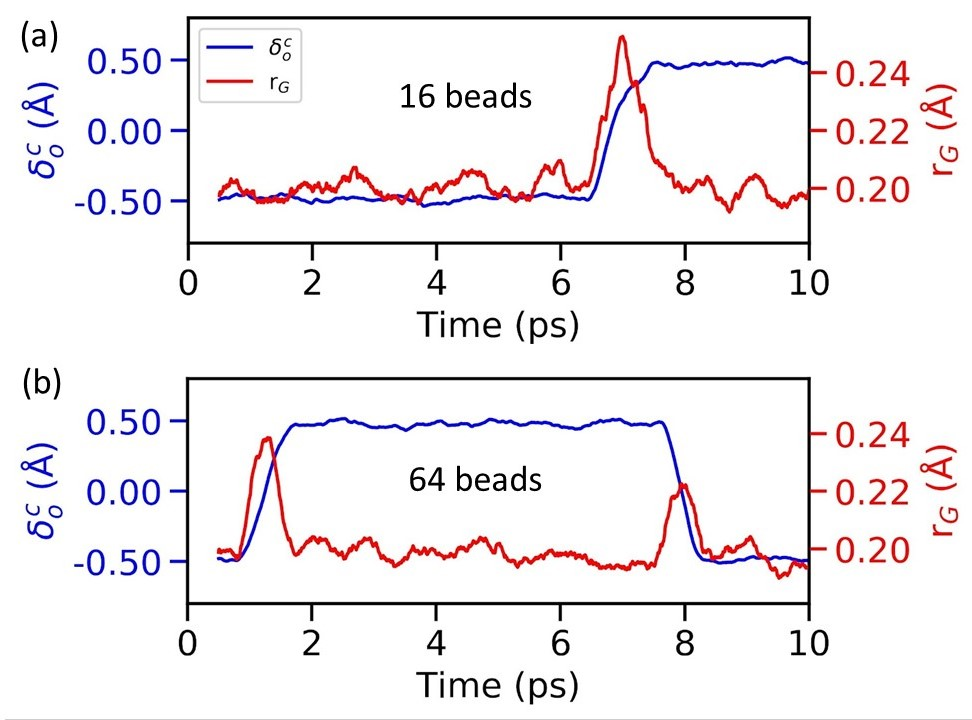
\includegraphics[width=15cm ]{./Appendix4/new_figures_si/figure10.jpg}
    \caption{The time evolution of the centroid proton transfer coordinate ($\delta_{o}^{c}$) and the radius of gyration ($r_G$) for (a) 16 and (b) 64 beads.}
    \label{fig:cip10}
\end{figure}

\section{NQE and finite temperature effects on double proton transfers}

In Chapter-3 we have discussed the results only for 70 and 300 K. Here we show how the different
quantities associated with the DPT evolves with increase in temperature. Figure~\ref{fig:cip13} shows 
the temperature dependent evolution of the free energy surface as a function of $d_{O-O}$ and
the proton transfer coordinate $\delta_{1,2}$, as obtained from the BOMD and PIGLET simulations. $\delta_{1,2}$
has been described in Chapter-3. While, in the BOMD simulations proton 
transfers were not obtained until the system attains room temperature,
in the PIGLET
simulations even at 70 K there are proton transfer events. We observe that as the temperature is increased the free energy difference between the
two minima decreases. 

%\begin{figure}[!ht]
%    \centering
%    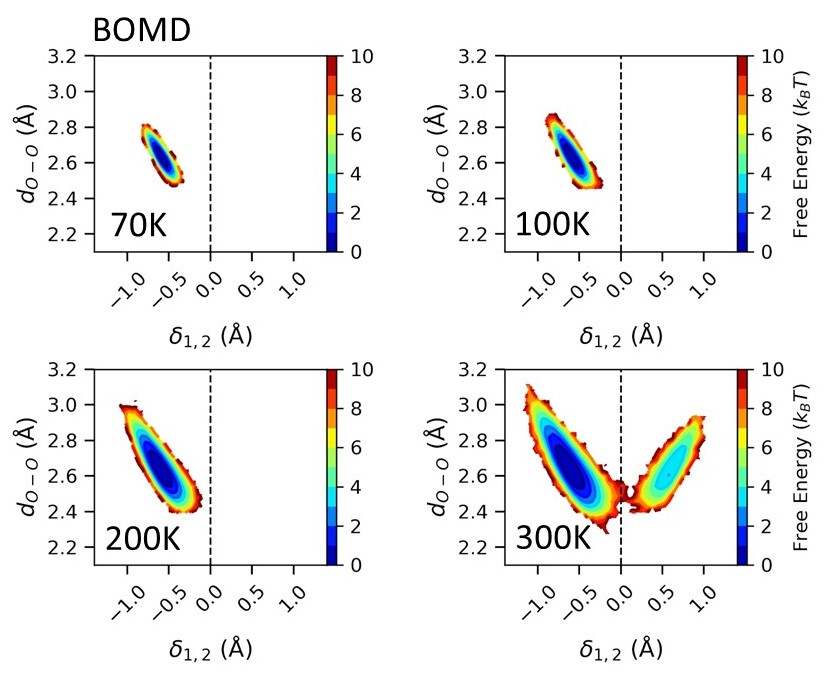
\includegraphics[width=15cm ]{./Appendix4/new_figures_si/figure3.jpg}
%    \caption{Temperature evolution of the effective free energy as a function of the proton transfer coordinate ($\delta_{1,2}$) and the heavy atom distance ($d_{O-O}$) obtained from BOMD simulations.}
%    \label{fig:cip3}
%\end{figure}

%\begin{figure}[!ht]
%    \centering
%    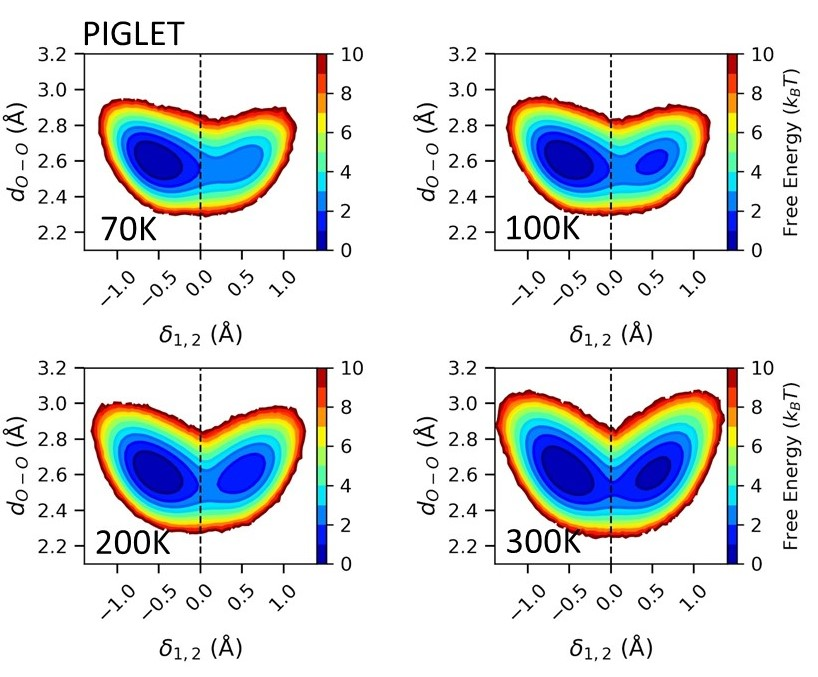
\includegraphics[width=15cm ]{./Appendix4/new_figures_si/figure4.jpg}
%    \caption{Temperature evolution of the effective free energy as a function of the proton transfer coordinate ($\delta_{1,2}$) and the heavy atom distance ($d_{O-O}$) obtained from PIGLET simulations.}
%    \label{fig:cip4}
%\end{figure}

\begin{figure}[!ht]
    \centering
    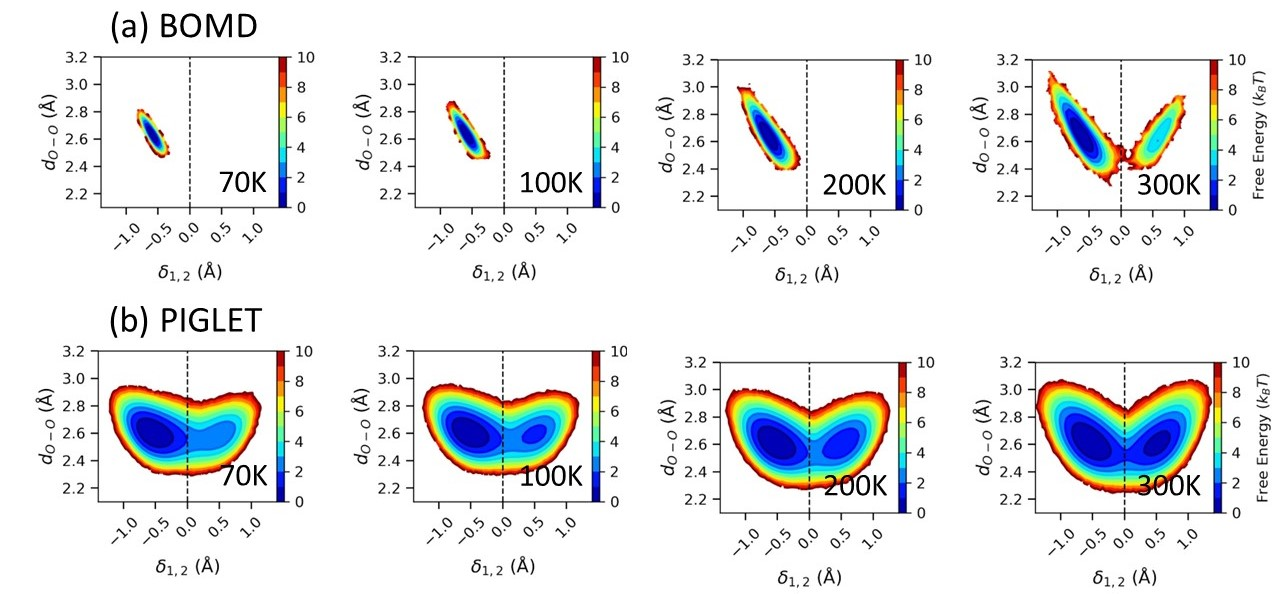
\includegraphics[width=16cm ]{./Appendix4/new_figures_si/figure_13.jpg}
    \caption{Temperature evolution of the effective free energy as a function of the proton transfer coordinate ($\delta_{1,2}$) and the heavy atom distance ($d_{O-O}$) obtained from (a) BOMD and (b) PIGLET simulations.}
    \label{fig:cip13}
\end{figure}

In order to investigate whether the double proton transfers are
stepwise or concerted, we have plotted the free energy surface as a function
of the proton transfer coordinates $\delta_1$ and $\delta_2$. Figure~\ref{fig:cip14}
shows the results obtained from BOMD and PIGLET simulations.

%\begin{figure}[!ht]
%    \centering
%    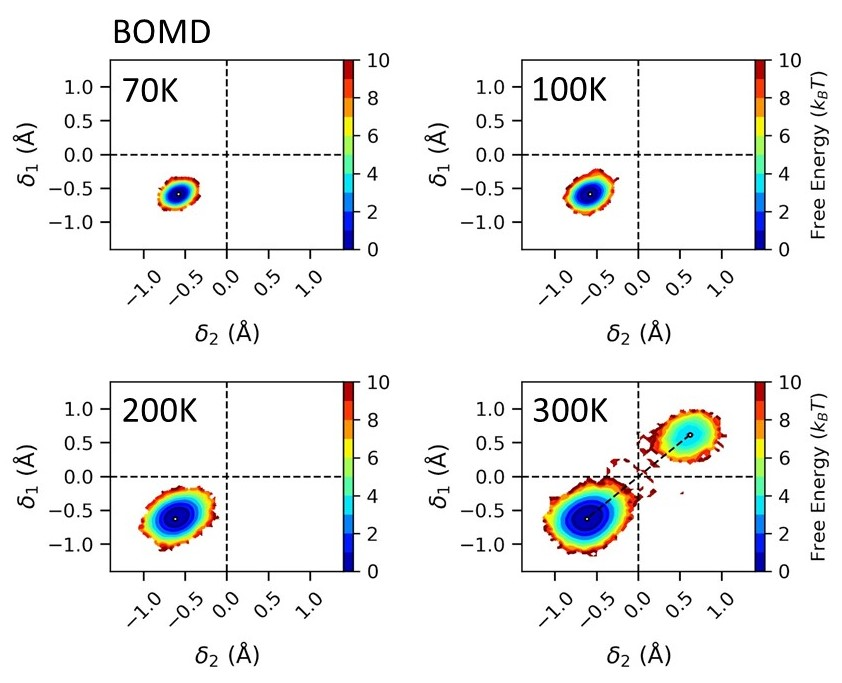
\includegraphics[width=15cm ]{./Appendix4/new_figures_si/figure5.jpg}
%    \caption{Temperature evolution of the effective free energy as a function of the proton transfer coordinates $\delta_1$ and $\delta_2$ obtained from BOMD simulations.}
%    \label{fig:cip5}
%\end{figure}

%\begin{figure}[!ht]
%    \centering
%    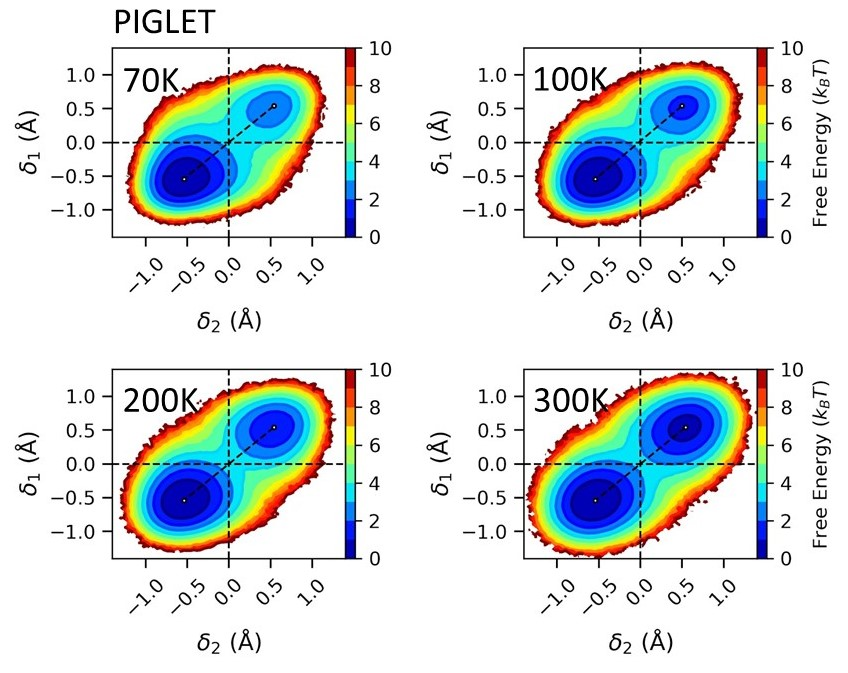
\includegraphics[width=15cm ]{./Appendix4/new_figures_si/figure6.jpg}
%    \caption{Temperature evolution of the effective free energy as a function of the proton transfer coordinates $\delta_1$ and $\delta_2$ obtained from PIGLET simulations.}
%    \label{fig:cip6}
%\end{figure}

\begin{figure}[!ht]
    \centering
    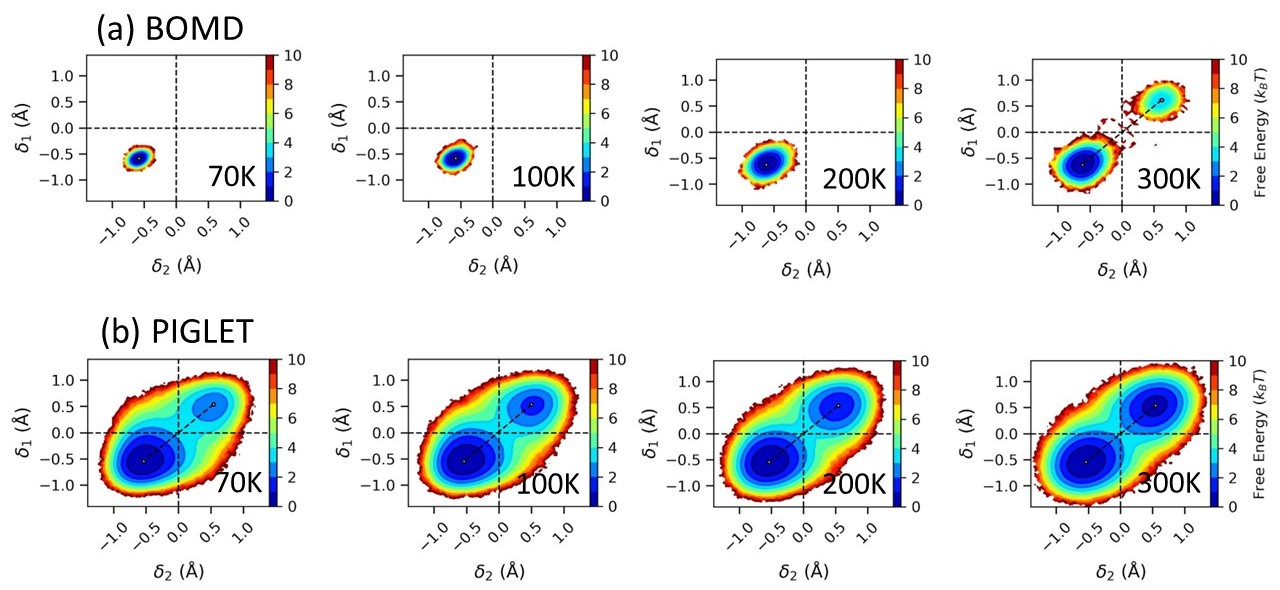
\includegraphics[width=16cm ]{./Appendix4/new_figures_si/figure_14.jpg}
    \caption{Temperature evolution of the effective free energy as a function of the proton transfer coordinates $\delta_1$ and $\delta_2$ obtained from (a) BOMD and  (b) PIGLET simulations.}
    \label{fig:cip14}
\end{figure}

Figure \ref{fig:cip11} displays the joint density plots of $\delta^c_o$ (centroid proton transfer coordinate) and $r^{\parallel}_G$ (component of $r_G$ parallel to the O-H bond) of the transferring protons as a function of temperature. The increase in temperature from 70 to 300 K leads to the gradual decrease in the spread of the joint distribution around $\delta^c_o = 0.00$. This behaviour reflects the gradual shift in the nature of the proton transfer from tunneling to activated hopping.

\begin{figure}[!ht]
    \centering
    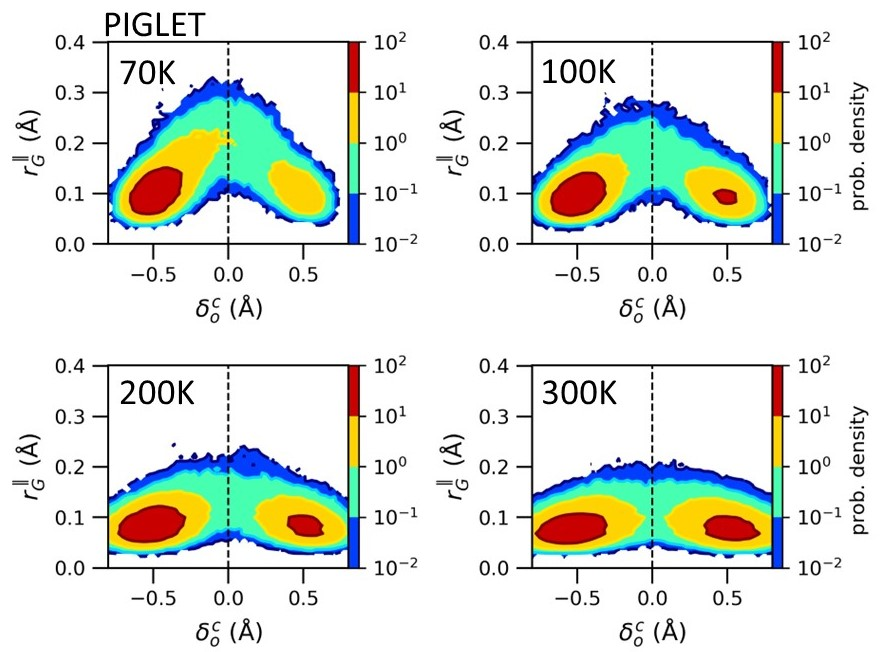
\includegraphics[width=15cm ]{./Appendix4/new_figures_si/figure11.jpg}
    \caption{Temperature evolution of joint distribution of $\delta^c_o$ and $r^{\parallel}_G$ obtained from PIGLET simulations.}
    \label{fig:cip11}
\end{figure}

\section{Weak improper \texorpdfstring{$C-H--O$}{} hydrogen bonds and its connection to the asymmetry of the DPT} \label{whb-td}

In addition to the intrachain strong H-bonds, the TPA crystal also has two weak interchain  $C-H\cdots O$ H-bonds (wHB1 and wHB2) as shown in Figure~\ref{fig:cip12}(a). The respective oxygen heavy atoms for the two wHBs have different bond order which dynamically depends on the position of the proton along the stronger $O-H\cdots O$ bond. Therefore, we plot the joint distribution between the wHB distance ($d_{H1-O1}$ in green and $d_{H2-O2}$ in red) and the proton transfer coordinate ($\delta_{1,2}$) in Figure \ref{fig:cip12}. Irrespective of the temperature and the NQEs effect, we observe that for $\delta_{1,2} < 0$, the two wHB distances ($d_{H1-O1}$ and $d_{H2-O2}$) are different where the shorter (longer) wHB is created from the \textit{sp$^3$} (\textit{sp$^2$}) hybridized carboxyl oxygen. On the other hand for $\delta_{1,2} > 0$, the bond order of the two different O heavy atoms interchanges but the corresponding wHB distances do not interchange and attain similar values due to the packing of the crystal. This creates a difference in the crystal environment when the proton is situated at $\delta_{1,2} < 0$ and when it present at at $\delta_{1,2} > 0$. Therefore, the proton experiences an asymmetric potential along the  $O-H\cdots O$ bonds and the DPT produces non-degenerate tautomers. It is to be noted that in the case of gas phase TPA dimer the tautomers are degenerate at 0 K as the crystal fields ($C-H\cdots O$ interactions) are non-existent. 

\begin{figure}
\centering
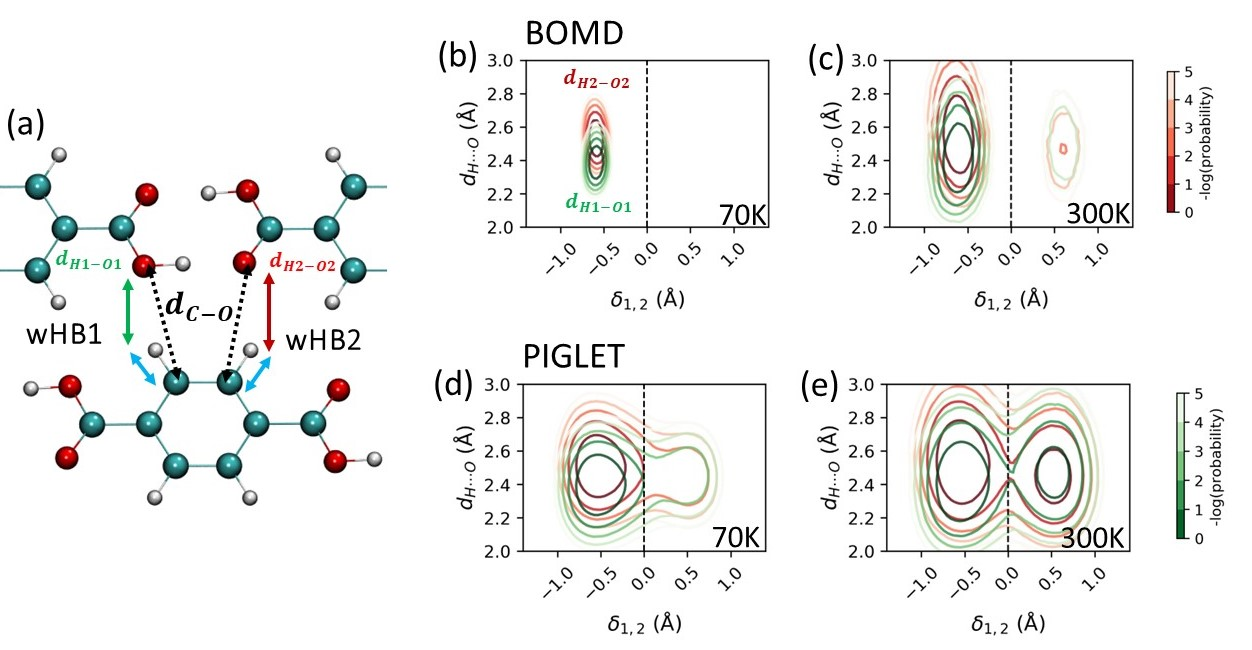
\includegraphics[width=15cm ]{./Appendix4/new_figures_si/figure12.jpg}
\caption{The joint density distribution between the wHB ($d_{H1\cdots O1}$ in green and $d_{H2\cdots O2}$ in red) with the proton transfer coordinate ($\delta_{1,2}$) obtained from the BOMD (a and b) and PIGLET (c and d) simulations at 70 and 300 K.}
\label{fig:cip12}
\end{figure}

\section{Correlation between the proton transfers during DPT in imaginary time}
\label{losss}

DPT in both the classical and quantum nuclei simulations are concerted as the anti-parallel transfers of hydrogen atoms is synchronous (Figure \ref{fig:delta1_delta2}). However, the PIGLET simulations show finite proportion of events in the second and fourth quadrant of the joint distribution. These events indicate the presence of high energy charged intermediates. In order to understand the exact nature of this small but finite events, we compute the mean deviation (represented by $\Delta$) of the two hydrogen transfer coordinates ($\delta_1$ and $\delta_2$) from the global proton transfer coordinate ($\Phi$) as a function of the imaginary time ($\tau$) slice or bead. 
\begin{equation}
    \Delta = (\frac{1}{2} (\delta_1-\Phi)^2 + \frac{1}{2} (\delta_2-\Phi)^2)^{\frac{1}{2}},{}{} \Phi = \frac{1}{2} (\delta_1 + \delta_2)
\end{equation}

Since the sampling involves multiple DHTs we plot the mean of $\Delta$ ($<\Delta>$) as a function of imaginary time. Moreover, $<\Delta>$ are calculated for two regions of the global proton transfer coordinate of the centroid path ($\Phi^c$) namely ``minima" where both the transferring proton are at the minimum of the potential energy surface experienced by the respective proton (-0.55 $ < \Phi^c < $ -0.45 and 0.45 $ < \Phi^c < $ 0.55) and ``saddle" where the protons are near the center/transition state (-0.2 $< \Phi^c <$ 0.2). The temperature dependent values of  $<\Delta>$ as a function of imaginary time slice is shown in Figure \ref{fig:imagine}. In the case of complete correlation the value of $<\Delta>$ is zero. However, due to temperature effects and zero point energy the values are generally higher than zero. The values of $<\Delta>$ for the protons near the ``minima" are used as a reference to account for the the temperature and zero-point effects. At 70 K, we find the $<\Delta>$ near the minima of the wells have values close to 0.1 \AA{} for all imaginary time slices and therefore serves as an internal reference. Near the saddle point, the value of $<\Delta>$ at $\tau=0$ is relatively higher $\sim$ 0.2 \AA{} whereas $<\Delta>$ at other values of $\tau$ is close to the values found around the minima. As the temperature increases, $<\Delta>$ ($\tau=0$) reduces whereas $<\Delta>$ ($\neq$0) increases to values $\sim$ 0.15 \AA{}. Therefore, in either cases the DPTs are concerted  but not correlated as found for formic acid dimer\cite{ivanov2015quantum}. At 70 K, the loss of correlation is due to tunneling achieved by increase of $<\Delta>$ at $\tau=0$ which manifests as an enhanced elbow observed in the second and fourth quadrant in the joint distribution of $\delta_1$ and $\delta_2$ (Figure \ref{fig:delta1_delta2}, PIGLET). However, at 300 K, the loss in correlation of the transferring hydrogen atoms are same for all imaginary time slices and is observed mostly due to thermal effects. This concludes that though the DPTs mostly generate neutral tautomers but also produces small proportion of charged intermediates.

\begin{figure}
    \centering
    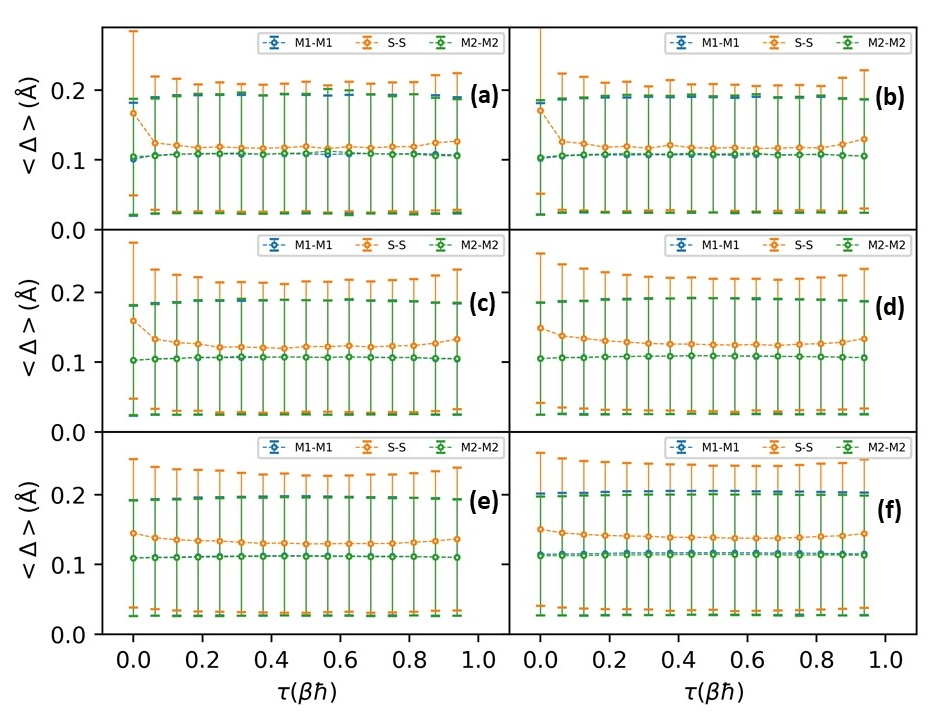
\includegraphics[width=15cm ]{./Appendix4/new_figures_si/imagine.jpg}
    \caption{Temperature dependence ((a) 70 K and (b) 300 K) of $<\Delta>$ plotted as a function of imaginary time slices ($\tau$).}
    \label{fig:imagine}
\end{figure}
